\documentclass{template}
\usepackage{graphicx,parskip,appendix,float,geometry}

\usepackage[
    backend=biber,
    style=ieee,
  ]{biblatex}
  \addbibresource{thesis.bib}
 % NOTE: https://www.overleaf.com/learn/latex/Biblatex_bibliography_styles
 % NOTE: Font Sizes https://en.wikibooks.org/wiki/LaTeX/Fonts

\geometry{
 a4paper,
 total={150mm,240mm},
 left=35mm,
 top=25mm,
 }

\renewcommand*\familydefault{\sfdefault}
\usepackage[T1]{fontenc}

%  http://tex.stackexchange.com/questions/86120/font-size-of-figure-caption-header
\usepackage[font=small]{caption}

\usepackage[ruled] {algorithm2e}
\usepackage{url,amsmath,amssymb,fancybox,listings,pdfpages,caption,multicol,datetime,rotating, booktabs}
%\usepackage[usenames,dvipsnames]{color}
\usepackage[pagebackref=false,pdffitwindow=true]{hyperref}

% NOTE: The hyperref usepackage should be the last \usepackage!!
% NOTE: When pagebackref=true an error will appear at the end of compiling. press `q' to ignore
% NOTE: Referencing Algorithms does not work if this usepackage is before the hyperref include.!!
% NOTE: This is a comment, ignored when the document is compiled
% NOTE: The following document configuration settings generally do not need to be modified
% NOTE: More packages may need to be added to provide additional functionality

% NOTE: http://tex.stackexchange.com/questions/7546/how-to-get-latex-symbol-in-document
\definecolor{colBackGrnd}{rgb}{1,1,0.8}
\definecolor{colKeys}{rgb}{0,0,1}
\definecolor{colIdentifier}{rgb}{0,0,0}
\definecolor{colComments}{rgb}{0,.5,0}
\definecolor{colString}{rgb}{0,0,1}
\definecolor{colWhite}{rgb}{1,1,1}

\newcommand{\MyHookSign}{\hbox{\ensuremath\hookleftarrow}}

\newtheorem{Theorem}{Theorem}
\newtheorem{Proposition}[Theorem]{Proposition}
\newtheorem{Lemma}[Theorem]{Lemma}
\newtheorem{Proof}[Theorem]{Proof}
\newtheorem{Remark}[Theorem]{Remark}
\newtheorem{Claim}[Theorem]{Claim}
\newtheorem{Example}[Theorem]{Example}
\newtheorem{Definition}[Theorem]{Definition}

% NOTE: Setup for including program listings
\lstset{%
    float=H,
    basicstyle=\ttfamily\footnotesize,
    identifierstyle=\color{colIdentifier},
    keywordstyle=\color{colIdentifier}, %
    stringstyle=\color{colIdentifier},
    commentstyle=\color{colIdentifier}, %
    columns=flexible,
    tabsize=2,
    frame=single,
    extendedchars=true, %
    showspaces=false,
    showstringspaces=false,
    numbers=left, %
    numberstyle=\footnotesize,
    breaklines=true,
    prebreak={\space\MyHookSign},
    language=Java,
    backgroundcolor=\color{colBackGrnd},
    breakautoindent=true, %
    captionpos=b%
} % \hypersetup{colorlinks=true, citecolor=\color{colIdentifier}}

\sloppy % NOTE: To ensure the Right Hand Margin is used (Especially for long URLS)

\newcommand{\latex}{\LaTeX\ }
\newcommand{\authorName}{Author Name}
\newcommand{\reportTitle}{Report Title}
\newcommand{\degreeAward}{BSc in Computer Science } 

\hypersetup{
    pdftitle    = {\reportTitle},
    pdfauthor   = {\authorName},
    pdfsubject  = {Computer Science},
    pdfkeywords = {Comma separated list of keywords},
    colorlinks  = true, anchorcolor = blue, filecolor = blue, urlcolor = blue,
    linkcolor   = blue,    % NOTE: change (blue) to (colIdentifier) to have links within the document in Black
    citecolor   = blue,    % NOTE: change (blue) to (colIdentifier) to have citation links within the document in Black
}

% NOTE: END of the document configuration settings

\begin{document}

\DeclareGraphicsExtensions{.jpg,.png,.gif,.pdf}
% NOTE: When inserting Figures if the extension of the graphic file is not provided LaTeX will automatically search for the extensions declared above, in the order declared.

\title{\huge{\reportTitle}}
\author{\authorName}
\degreetitle{\degreeAward} % Replace with appropriate degree
\rpttype{BSc}    % Replace PhD / MSc  / BSc.
\principaladviser{Dr. Daniel C. Doolan}

\beforeabstract
\prefacesection{Abstract}
The Abstract of the report should be written here, it should provide a short summary of the work encompassing no more than one page.

\prefacesection{Acknowledgements}
The Acknowledgements section may be used to thank your supervisor, friends, family, peers or any other applicable individuals or institutions.

\afterpreface \afterabstract

\listofalgorithms   % NOTE: Will generate a list of Algorithms in the Table of Contents Section
\lstlistoflistings  % NOTE: Will generate a list of Program Listings in the Table of Contents Section

% NOTE: Include the relative reference for each chapter to be included dividing the thesis file structure into a number of directories aids development format: directory Name/filename (the .tex extension is not required for the filename)

\chapter{Introduction}
\pagenumbering{arabic} \setcounter{page}{1}

A short paragraph introducing the topic the chapter examines.


\section{Background}

A number of pages about the background of the project.

\section{About this Thesis}
This is the report of \emph{\authorName}, submitted as part of the requirements for the degree of \degreeAward \space at the \dept, \university, \universityLocation.

A number of paragraphs detailing the main expectations of this body of work.


\section{Chapter List}
Provide a list of all the chapters within the report and a brief summary of the content. Ensure each summary avoids having a repetitive structure such as starting with ``This chapter deals with''.

\textbf{Chapter \ref{ch:usingLatex}} Using \LaTeX. Explores the essentials one needs to know so a \LaTeX \space based report can be compiled and edited.

\textbf{Chapter \ref{ch:litReview}} Literature Review. Short summary of key points $\ldots$.

\textbf{Chapter \ref{ch:Background}} Background Research. Overview of chapter $\ldots$.

\textbf{Chapter \ref{ch:Design}} Design. Outline of the chapter $\ldots$.

\textbf{Chapter \ref{ch:Implementation}} Implementation. Main achievements actioned $\ldots$.

\textbf{Chapter \ref{ch:Evaluation}} Evaluation \& Testing. Did the artefact perform as required, $\ldots$.

\textbf{Chapter \ref{ch:Conclusion}} Conclusion. Summary of the journey and future directions $\ldots$.


\section{Conclusion}
A short conclusion summarising the chapter.

\chapter{Using \LaTeX}\label{ch:usingLatex}

By reading this chapter and comparing the generated output to the \latex code, one should be able to produce all the necessary content expected of a typeset report. Instructions regarding software installation and compilation are to be found towards the end of the chapter. As with any source code, one should first compile, it to ensure it works. This document should compile with no errors or warnings. 

The following sections provide some direction on how to typeset with \LaTeX. Word processing applications utilising  a ``What You See Is What You Get'' (WYSIWYG) type user interface (``Word'' / ``Writer'') are designed for general purpose use. Such applications are not designed for the creation of professional documents and reports requiring high levels of precision to ensure all elements from the individual characters of a word to the placement of tables and figures are presented as they should be. 

A key advantage of \latex is the decoupling of the content from the presentation. This inherently allows one to focus on what is of greatest importance, the content. With \latex one can write code akin to the HTML and CSS relation of decoupling content from presentation, the result of which can be compiled into a professionally typeset document, be it a report, cv, presentation or poster for example. When one needs to develop a professional and structured document then the ``You Asked For It You Got It'' (YAFIYGI) route that many in computing, maths and physics embrace is the generally preferred solution toward achieving a timely and high quality output. 

\clearpage

\section{Structure of this Template}
The file {\tt thesis.tex} in the root of the directory (ThesisTemplate) is the main file of this template. This is the file that must be compiled to create the document. The {\tt thesis.tex} document contains a lot of configuration settings. The only elements that require editing are details such as the title of the report, authors name and so forth. The only further addition to the file is to use the \emph{\textbackslash include} statement to include additional chapters in the report. One may also comment out the \emph{\textbackslash include} statements using the percentage sign (\%) to develop the report on a chapter by chapter basis. The BibTeX database {\tt thesis.bib} is also included within the root. All the actual content of the report is divided into directories each with a {\tt .tex} file containing the chapter content. Appendix~\ref{fig:append:TemplateStructure} provides a visual outline of the file and folder structure.

\section{Adding Figures to the Report}
The example below (Figure~\ref{fig:using:samplepngImage}) features a bitmap image. One can see that the extension for the image file isn't specified, as this template is setup to automatically search for .jpg, .png, .gif and .pdf images. To add a figure / image one should replicate the code in this subsection, which generates Figure~\ref{fig:using:samplepngImage}. One should then modify the \textbf{label}, \textbf{caption} and \textbf{image file name} to suit. The size of the displayed image within the document can be varied by adjusting the height and width attributes. To rotate an image 90 degrees an optional attribute can be added, for example [width=.4\textbackslash linewidth, angle=90].

\begin{figure}[H]
\begin{center}
\includegraphics[width=.34\linewidth]{usingLatex/images/samplepng}
\caption{Caption for Bitmap Image Example} \label{fig:using:samplepngImage}
\end{center}
\end{figure}

 One can insert graphic elements using \latex in a number of ways. Vector based imagery such as diagrams saved to the pdf format may use the \emph{\textbackslash includegraphics} command with the optional \emph{viewport} attribute to specify a precise area of the graphic to be included. Figures should also include a Caption and a Label for referencing.

When inserting a Figure (Figure~\ref{fig:using:VectorGraphicElementPDF}) one uses the \emph{\textbackslash begin\{figure\}} and \emph{\textbackslash end\{figure\}} commands. The image presented is a vector graphic in the form of a pdf file. When working with such files it is usually necessary to include the optional \emph{viewport} attribute to designate the specific area in which to focus. The first pair of coordinates (x~\&~y) designate the pixel location of the lower left corner. The second pair identify the upper right hand corner. Modification of these coordinates allows one to focus in upon a particular area of interest within the vector image. 


\begin{figure}[H]
\centering
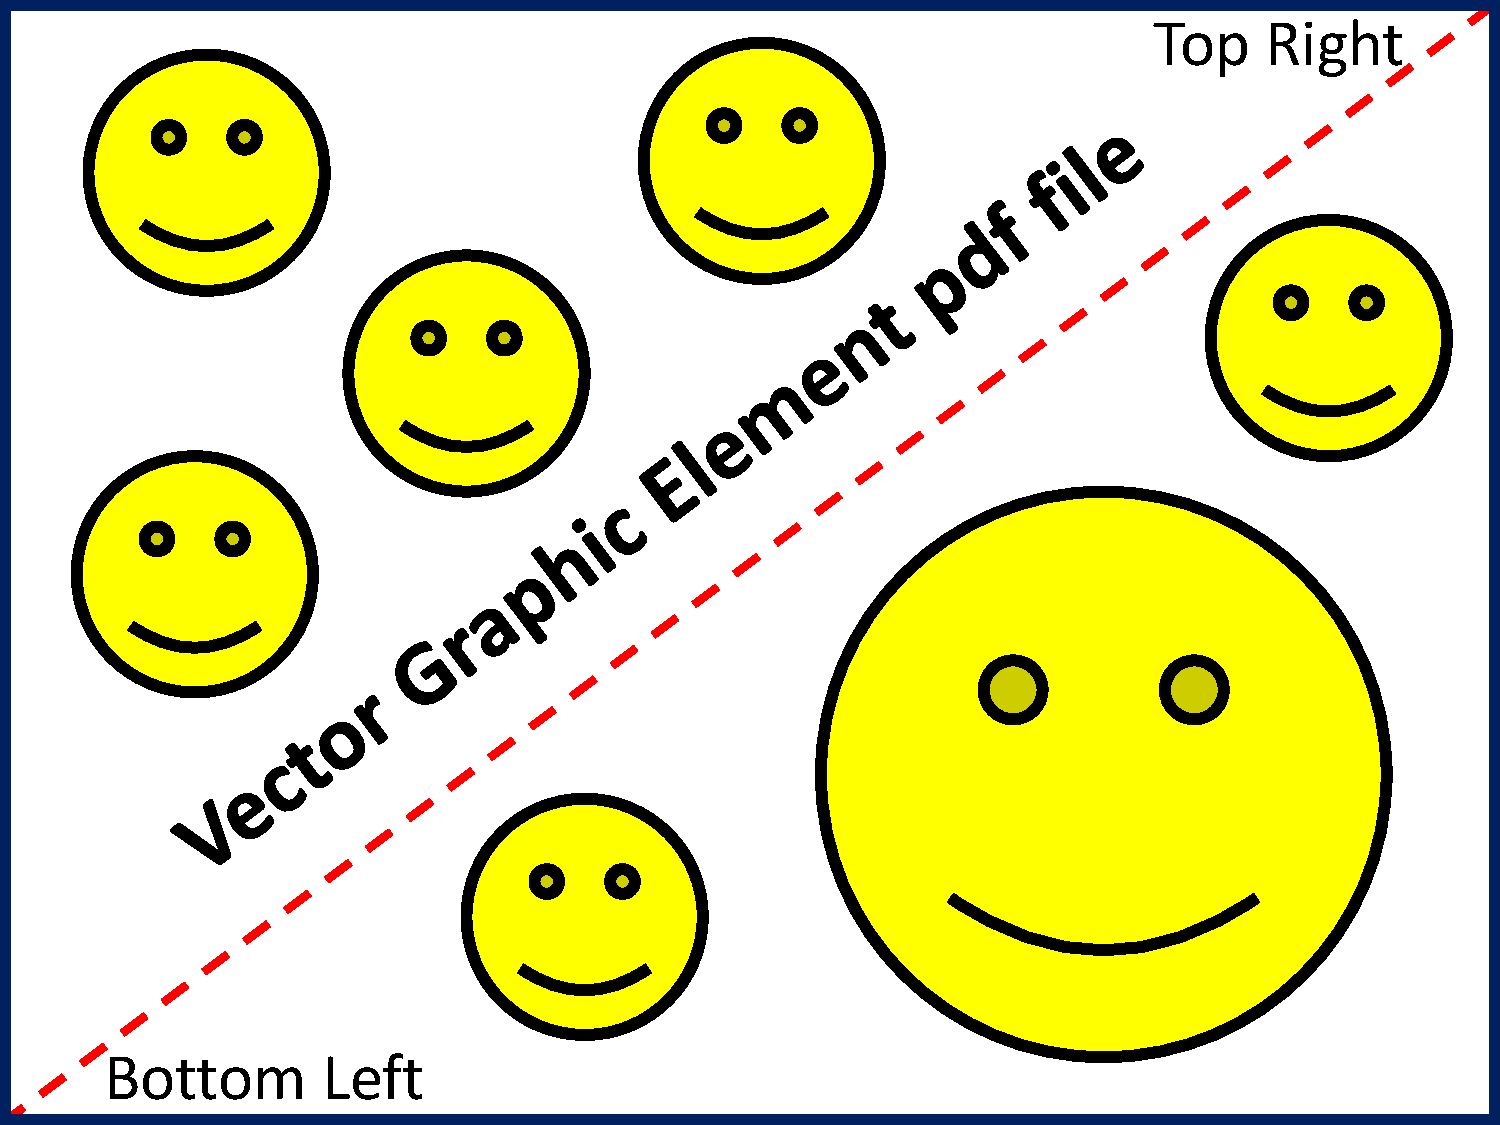
\includegraphics[width=.4\linewidth]{usingLatex/images/VectorGraphicElementPDF.pdf}
\caption{Vector Graphic - pdf of a PowerPoint Slide}
\label{fig:using:VectorGraphicElementPDF}
\end{figure}

The optional attribute [H] when beginning a Figure inserts the graphic element at the specified location. Other options such as [htb] (here, top, bottom) will place the graphic in the most suitable place that \latex can find. This however can have a negative impact on memory allocation if a large number of images exist, therein preventing compilation.



One may use the \emph{minipage} command when inserting two figures to span across the page. This allows for the subdividing of the page into a number of columns of specified width. Figure~\ref{fig:using:Example1} \&~\ref{fig:using:Example2} illustrate how one may zoom in / focus on a particular section of a graphic by altering the coordinates of the \emph{viewport}. 

\begin{figure}[H]
\begin{minipage}[t]{7.4cm}
\begin{center}
\includegraphics*[viewport= 20 20 600 440, width=.8\linewidth]{usingLatex/images/VectorGraphicElementPDF.pdf}
\caption{Viewport = 20 20 600 440}
\label{fig:using:Example1}
\end{center}
\end{minipage}
\hfill
\begin{minipage}[t]{7.4cm}
\begin{center}
\includegraphics*[viewport= 220 200 400 330, width=.8\linewidth]{usingLatex/images/VectorGraphicElementPDF.pdf}
\caption{Viewport = 220 200 400 330}
\label{fig:using:Example2}
\end{center}
\end{minipage}
\end{figure}

\clearpage
The key advantage to using vector imagery for diagrammatic and textual content is that such imagery contains embedded instruction on what is to be drawn, therefore it can scale to any size without loss of image quality. This contrasts with a bitmap or raster image which results in a matrix / array of pixel values. If saving a screenshot then  .png is preferable over a .jpg which is a lossy file format yielding many artefacts with image content which transitions rapidly, such as from text or a line to a background.

\section{Referencing Another Element of the Report}

To refer to another part of the document one must use a combination of the \emph{\textbackslash ref} and \emph{\textbackslash label} commands. The label is a unique identifier, therefore when working with large documents it helps to give references meaningful names. Examples of this includes prefixing Table references with \emph{tab:}, figures with \emph{fig:}, chapters with \emph{ch:}. In very large documents in may also be useful to add an additional level of prefixing to represent the chapter the label is in. In this example chapter the tables and figures have the additional prefix of \emph{using} to represent the \emph{usingLatex} chapter. The tilde ($\sim$) known as a ``tie'' in \latex is used to ensure that a reference remains as a single unified object. All instances of \emph{\textbackslash ref} should be preceded with the tilde. Section~\ref{using:sec:WorkWithMath} refers to ``Working with Mathematics'' identified with \emph{\textbackslash label$\{$using:sec:WorkWithMath$\}$} right after the section heading and referred to here via the instruction \emph{Section$\sim$\textbackslash ref$\{$using:sec:WorkWithMath$\}$}.

\section{Citing Bibliographic References}
Bibliographic references are stored in a database (.bib file extension), this contains a list of articles, proceedings, books, thesis and online information sources. Each type of publication has a number of required fields such as a unique identifier, author and title. To cite a reference within the main body text one must use the \emph{\textbackslash cite} command as per the following examples. Donald Knuth \cite{book:knuth_1973} for example is well known for his work on the Art of Computer Programming. The SETI@Home project \cite{online:berkeleyBOINC} is an example of a webpage citation. One can also work with articles \cite{art:Russell:1978:Cray1}, MSc Thesis \cite{msc:Shannon:1940}, PhD Thesis \cite{phd:Sutherland:1963} or articles within conference proceedings \cite{proc:Ewald:1978:HPG}. Dr. Doolan \cite{online:Doolan:2016:AcademicResources} has provided an online list of resources that may be useful for undertaking literature reviews, along with a number of useful templates, \latex tools and necessary software. These citations were made using the \emph{\textbackslash cite\{bibEntryReference\}} command. 

\subsection{Specifying Pages or other Elements within a Reference}
To refer to a particular page, section, chapter, equation or other element of a large document add the corresponding information within square brackets right after the \emph{\textbackslash cite} command, such as \emph{\textbackslash cite[p. 2]$\{$online:IEEE-ReferenceGuide:2018$\}$}. Further information is available from the ``IEEE Reference Guide'' \cite[p.3]{online:IEEE-ReferenceGuide:2018}, located in section I.B \cite[Sec I.B]{online:IEEE-ReferenceGuide:2018}. Table~\ref{tab:ReferenceExamples} illustrates a number of common elements one may refer to within a citation, in this case pages or elements of reference ``42'' \cite[Ch. 27]{book:Adams:1979}.

\begin{table}[H]
\caption{Examples of References within a Reference}\label{tab:ReferenceExamples}
\centering
\small
\begin{tabular}{ll}
\toprule \textbf{Reference Type}& \textbf{Presentation Format}\\
\midrule
A Single Page & [42, p. 8] \\
Range of Pages & [42, pp. 4-8] \\
Figure & [42, Fig. 8] \\
Table & [42, Tab. 4] \\
Appendix & [42, Appendix. F] \\
Specific Section & [42, Sec. 4.8] \\
Chapter and Pages & [42, Ch. 4 pp 42-64] \\
An Algorithm & [42, Alg. 4] \\
An Equation & [42, eq. (4)] \\
\bottomrule
\end{tabular}
\end{table}

\subsection{Referencing Style}
Quite a number of Universities use the ``Harvard'' referencing style, this makes use of the author name and date in the body text of the report to make a citation. The references generally found at the end of the report are sorted by author name. Several subject disciplines regularly use the Harvard format such as the arts, humanities and business. This is fitting with a more discursive narrative common amongst those subject areas. 

It is always useful to check the University Referencing Style Guide for your institution. You will find that the University Library provides detailed information and examples on how to reference. Many University Style Guides may suggest Harvard as the institutional standard, however they may also stipulate the use of the most appropriate style for the discipline. The IEEE Referencing Style in this template is regularly used in Computing.      

In Computing it is far more common to see citations in the body text represented as a number within square brackets. The associated references are listed in the order they appear within the body text, preceded with the associated reference number. An advantage with this referencing style is far less real-estate being occupied by the citation. 

\subsection{Compiling a BibTeX Database}

Having initially compiled the document using pdfLatex on your local machine making use of a \latex distribution and a front end editor a number of helper files are created that aid in referencing and citations. One must the compile the bibtex database, followed by an additional two compiles using pdfLatex. Citing additional bibliographic references within the body of the document being produced will require the recompile of the bibtex database. In the case that the bibtex reference of a cited article cannot be found one will see a question mark (?) instead of the proper citation and a compile warning.

\section{Working with Mathematics}\label{using:sec:WorkWithMath}
The power of \latex in typesetting mathematical formula is one of its key strengths. The mathematical definition of the ``Cantor set'' is a good example of this in action encompassed within an \emph{\textbackslash equation} environment.

\begin{equation}
\displaystyle\sum_{n=0}^\infty \frac{2^n}{3^{n+1}} = \frac{1}{3} +
\frac{2}{9} + \frac{4}{27} + \frac{8}{81} + \cdots =
\frac{1}{3}\left(\frac{1}{1-\frac{2}{3}}\right) = 1
\end{equation}
 The previous equation demonstrates the use of sigma, fractions, large brackets, power, and dots. The function that defines the MSet $Z_{n+1} =
Z_{n}^2 + C$ is a simpler example of math in use within the body text of a paragraph. Matrix Multiplication is typically regarded as an $O(n^3)$
operation. One may use the \emph{equation} environment for more complex mathematical formula that should standout. For example the product  $C$ of two matrices $A \in M_{n,m}(R)$ and $B \in
M_{m,p}(R)$ may be defined as

\begin{equation}
(A \times B)_{ij} = \sum_{k=0} ^{m-1} a_{ik}b_{kj},~
i=0,...,n-1,~j=0,...,p-1.
\end{equation}

The sizes of the matrices must satisfy $(n \times m)(m \times p) =
(n \times p)$. Matrix multiplication is an associative process
thereby $a\cdot(b \cdot c) = (a \cdot b) \cdot c$. Essentially to
find the value of a particular cell $C_{i,j}$ it is necessary to
multiply row $i$ of the matrix $A$ with column $j$ of matrix $B$
summing all the multiplications.

\clearpage
\section{Inserting an Algorithm}

The \emph{algorithm2e} environment \cite{online:Fiorio2016algorithm2e} may be used to generate algorithms (Algorithm~\ref{alg:using:SampleAlgorithm}). If no algorithms are used within the document then comment out \emph{\textbackslash listofalgorithms } in the file {\tt thesis.tex} to remove the list of algorithms page.

\begin{algorithm}
%\dontprintsemicolon
\While{(RANK $<$ COMPSIZE)}{
    \If{(RANK == MASTER)}{
        generate random value \;
        \For{(each item K)}{
            get result \;
        }
    }
}
\caption{A Sample Algorithm} \label{alg:using:SampleAlgorithm}
\end{algorithm}


\section{Adding a Table with the Tabular Environment}

The cells in Table~\ref{tab:using:TableExample} displays three columns of left-aligned and one column of justified data. The cell contents can be aligned to the left (l), right (r), center (c) or (p). Vertical bars may sometimes be seen in tables but these generally look unprofessional. The Booktabs package \cite{online:Fear2016BookTabs} allows for the creation of professional looking tables as shown in the example.  The use of \emph{\textbackslash toprule}, \emph{\textbackslash midrule} and \emph{\textbackslash bottomrule} commands provided by the package allow for rules of varying thickness and spacing. Data elements (cells / columns) within a table are divided up using the ampersand (\&). Completion of a row ends with a double backslash (\textbackslash\textbackslash). Tables as with figures need a caption and a label. The WinShell editor has a GUI based utility to aid in the creation of the tabular data. Replicate the code in this subsection, which generates Table~\ref{tab:using:TableExample}. One should modify the \textbf{label}, \textbf{caption} and \textbf{content} of the table to suit.

\begin{table}[H]
\caption{Table Caption}\label{tab:using:TableExample}
\centering
\small
\begin{tabular}{lllp{5cm}}
\toprule \textbf{Heading 1}& \textbf{Heading 2}&\textbf{Heading 3}&\textbf{Heading 4}\\
\midrule
Cell A1 & Cell B2 & Cell C3 & Cell D4\\
Cell E1 & Cell F2 & Cell G3 & Justified text with a defined column size of 5cm\\
\bottomrule
\end{tabular}
\end{table}





\section{Inserting Program Code Samples}

To insert small segments of program code (Listing~\ref{code:SampleCode}) that detail how interesting algorithms and so forth are implemented use the \emph{lstlisting} command. Inclusion of program code again requires a Caption and Label. Sample code from external files may also be included (Listing~\ref{code:externalSampleCodeLabel}), by supplying the relative path to the source file. 

\begin{lstlisting}[caption=Sample Program Code Listing, label=code:SampleCode]
if(rndVal==0){
    if(opType > 2){
       //do something
    }
}
\end{lstlisting}

\lstinputlisting[caption={The Caption for the Code Listing},label={code:externalSampleCodeLabel}]{usingLatex/myCodeFile.java}

\section{Creating Numeric and Bulleted Lists}
Replicate the code in this subsection to create numbered or bulleted lists. As can be seen in the example below one can create different levels of list elements if necessary. Its best to limit the use of lists and focus more on paragraphs of text to convey the narrative of a report. Lists can sometimes be useful emphasise key elements. 

{\setstretch{0.85}% Reduces line spacing to compact the list items
\begin{enumerate}
\item First element of a numbered list
\item Second element of a numbered list
\end{enumerate}
\begin{itemize}
\item First element of a bulleted list
\item Second element of a bulleted list
    \begin{itemize}
    \item First nested element of a bulleted list
    \item Second nested element of a bulleted list
    \end{itemize}
\end{itemize}
} % Closing Parenthesis  with respect to the use of \singlespacing for the display of the list elements


\section{Using the Correct Quotes}
To surround a piece of text with double quotes one must place two single quotes on either side of the text. The double quote on the left is created using two left quotes (\lq) this is located just above the \emph{tab} key on the keyboard. The right hand double quote is created using two right hand quotes via (\rq) located just above and to the left of the right shift key. A properly formatted quotation should look like ``This is a quotation''. Notice how the direction of the quotes are opposite to one another. A larger example using the \emph{\textbackslash Huge} font size option, is presented below so the quotes can be clearly seen.

\begin{center}
\Huge{``This is a quotation''}
\end{center}

\section{Widows and Orphans Anomalies to Avoid}
These anomalies can occur at the paragraph and page level. A paragraph where a single word or two flows over on to a new line is inherently wasting valuable space on the page. It is thereby worthwhile to review and rephrase the paragraph to avoid such instances \textcolor{red}{occurring.}  

The paragraph above is a good example of such wasted space, take note of the last word of the paragraph ``occouring'', in essence it is positioned all alone, away from all the other words compromising the unit paragraph. Another example is where the starting line of a paragraph begins at the end of a page, with the bulk of the paragraph existing on the next page. Making use of \emph{\textbackslash clearpage} can often help, to push the entire paragraph on to the next page. Likewise the last sentence of a paragraph may run over onto the next page. One should review and rephrase the paragraph as needed to avoid this, therein maintaining the structural integrity and cohesiveness of the paragraph as a single unit. 

\section{What is a Paragraph}
All too often one sees paragraphs comprising of a single sentence, comprising a line or two. Such is inherently not a paragraph. A paragraph should ideally comprise around half a dozen plus sentences, focused on are particular topic of discussion. Often the starting sentence of the paragraph introduces the concept, while the last sentence concludes the discussion put forth. Hence a paragraph should be a cohesive unit of narrative unto itself. This paragraph, not withstanding this sentence, started out by outlining a common problem with paragraphs, then explained the expected structure and concluded that it should be a standalone unit of prose. 

\section{\latex Setup and Install on a Local Machine}
The implementation of \latex that is often used is MikTeX (\url{http://miktex.org}). It is typically best to install the complete MiKTeX  system. A complete system comprises of around 40K files. A minimal install will necessitate the installation of packages as needed. One can individually download and integrate packages into a MikTeX system using the ``Package Manager (Admin)'' application. Initially a small installer application must be downloaded and executed. This in-turn downloads the most recent implementation of the MikTeX system. Run the installer again and select the directory of the downloaded package. Mac users can use the MacTeX distribution (\url{http://www.tug.org/mactex/}). 

\subsection{Front End Editor}
Texmaker (\url{https://www.xm1math.net/texmaker/download.html}) is a very useful free GUI based editor that includes a built in document viewer. TeXnicCenter is a free download available at (\url{http://sourceforge.net/projects/texniccenter/}). An alternative is WinEdt a shareware ASCII editor (\url{http://www.winedt.com}). WinEdt can be freely used for a 30 day period, after which one will periodically receive reminders to register the product. WinShell (\url{http://www.winshell.de}) is another option for Windows users. An advantage of WinShell is its in-built BibTeX GUI editor. It also has a useful Table Wizard. TexShop (\url{http://pages.uoregon.edu/koch/texshop/}) is a popular option for Mac users, providing a very easy to use editor. Note the website links in this section were created using the \emph{\textbackslash url} command and included for ease of reference. 

\section{Start Compiling and Editing}
{\setstretch{0.98}
\begin{enumerate}
\item Read the instructions in this file thesisTemplate.pdf, compare the code in the file usingLatex.tex to that of the resultant output of the Using \latex chapter. 

\item Download and install the back-end \latex system and front-end text editor. 

\item Compile the files thesis.tex and thesis.bib to generate the file thesis.pdf so that it is identical to file thesisTemplate.pdf.
\begin{enumerate}
\item To achieve this compile with pdfLaTeX, then run BibTeX and compile with pdfLaTeX two further times.

\item It is only necessary to run BibTeX when new citations are added.

\item Two compiles of pdfLaTeX is sufficient to allow for correct reference  linkage.

\item If one is simply adding additional content (text / figures / tables) then a single compile of pdfLaTeX is sufficient for testing purposes.
\end{enumerate}
\item Several new files may now be seen in the ``ThesisTemplate'' root and subfolders. 

\item With a successful compile achieved, start reading through the \latex documents (.tex) to see how the various elements are assembled.

\item Begin editing the document starting with {\tt thesis.tex} by entering elements such as ``Thesis Title'' and ``Author Name''.

\item When it is necessary to start inserting figures / tables and so forth, copy and paste the \latex code provided and edit as necessary.
\end{enumerate}
} % END setstretch


\section{Conclusion  the \latex Advantage}
Having read this chapter and compared the {\tt .tex} source to the generated output, one should have all the knowledge necessary to typeset a well formatted and elegant project report. One needs to become familiar with a number of commands, but once mastered it should greatly speedup the report writing process. By using \latex to typeset a document one is removed from a myriad of issues in relation to formatting allowing one to concentrate on the most important task, that of content creation. 

By making use of \latex one can focus on the content. As one will see by compiling the source code of this document, all the material is laid out without having to spend significant amounts of time focused on the presentation elements. All the presentation elements from headings and section numbering are automatically generated, as are things such as report front matter, table of contents and references to highlight just a few.

\chapter{Background Research}\label{ch:Background}

This chapter provides some background research on the project and examines some previous work.

\section{Conclusions}

The main conclusions for this chapter.



\chapter{Literature Review}\label{ch:litReview}

This chapter provides a comprehensive review of the most relevant literature in the field showing how it feeds into the product being delivered. ``IEEE Xplore'', ``Google Scholar'' and the ``ACM Digital Library'' are examples of useful data sources that may be queried as part of the review process. Dr. Doolan \cite{online:Doolan:2016:AcademicResources} provides links to these and other resources. 

\section{Introduction}
Intro of topic discussion.

\section{Key Topic Area 1}
Section of topic discussion.

\section{Key Topic Area 2}
Section of topic discussion.

\section{Key Topic Area 3}
Section of topic discussion.

\section{Conclusions}

The main conclusions of the chapter.



\chapter{Design}\label{ch:Design}

This chapter examines the design of the project.

\section{Conclusions}

The main conclusions for this chapter.



\chapter{Implementation}\label{ch:Implementation}

This chapter examines the implementation of the project.

\section{Section Discussion Heading}

Section 1 implementation discussion.

\subsection{Subsection Heading}
Subsection paragraph text.

\section{Conclusions}
Conclusions paragraph text.






\chapter{Evaluation \& Testing}\label{ch:Evaluation}

This chapter evaluates the overall project and provides results of tests carried out.

\section{Conclusions}

The main conclusions for this chapter.



\chapter{Conclusion}\label{ch:Conclusion}

This chapter summarises the main positive outcomes and conclusions resulting from this body of work. One can explore the overall journey, problems encountered and solutions found. Of key importance is the ``Future Work'' section highlighting how the product may be further developed with new and improved features, futher resources and time. 

\section{Conclusions}

The main conclusions that may be drawn from the body of work.

\section{Future Work}

Further development that could be carried out in the future.


% NOTE: reduced the size of the text for the bibliography
% NOTE: set the style for the bibliography and display the references used within the document

% NOTE: http://tex.stackexchange.com/questions/67153/bibliography-not-in-toc-when-using-biblatex-biber
%\printbibliography[heading=bibintoc]
\footnotesize
\addcontentsline{toc}{chapter}{Bibliography}
\printbibliography

\normalsize
\appendix
\chapter{Project Specification}
Summary of the project outline.

\section{Functional Requirements}
Some text here.

\section{Non-Functional Requirements}
Some text here.

\chapter{Project Management}
Discussion on how the project was managed. What things impacted the success of the project. How does the continually revised versions of the project plan compare to the initial draft developed at the start of the project. Did everything run according to schedule. What impact did elements such as exams \& coursework have on the project. 

Undertaking a Project is a \textbf{Marathon not a Sprint}. Start immediately by firstly fully understanding what is required, start learning new languages, tools, technologies, libraries that you need and make a start on writing the report. Make full use of the time provided, making headway straight away, this will provide positive reinforcement and help propel the work along. A good analogy is that of the ``Gym'' or "DevGym" / ``Development Gym of Learning and Skills'' only by the investment of regular and consistent work, will results be achieved. As Gandalf eloquently puts it ``All we have to decide is what to do with the time that is given us'' \cite{book:Tolkien:1991:FOTR}\cite{online:Jackson:2001:FOTR}. 

Professor Randy Pausch is well known for his contribution to the ``Alice 3D'' environment as well as lectures on ``Time Management'' and ``Fulfilling your Childhood Dreams''. Both of these lectures are well worth watching, Dr. Doolan \cite{online:Doolan:2015:PauschLecture} outlines the main elements of both lectures. The post features a number of links allowing one to jump to particular segments of interest in the video lectures. Dr. Doolan \cite{online:Doolan:2016:SchwarzeneggerInterview} again highlights the key elements of success in the form of Goals, Confidence and Time Management. The post summarizes and highlights key elements of a video interview with Arnold Schwarzenegger.

\chapter{Another Appendix}

This appendix makes use of the \emph{rotating} package to rotate both figures and tables ninety degrees allowing for large datasets and illustrations to be represented.

\begin{figure}[H]
\centering
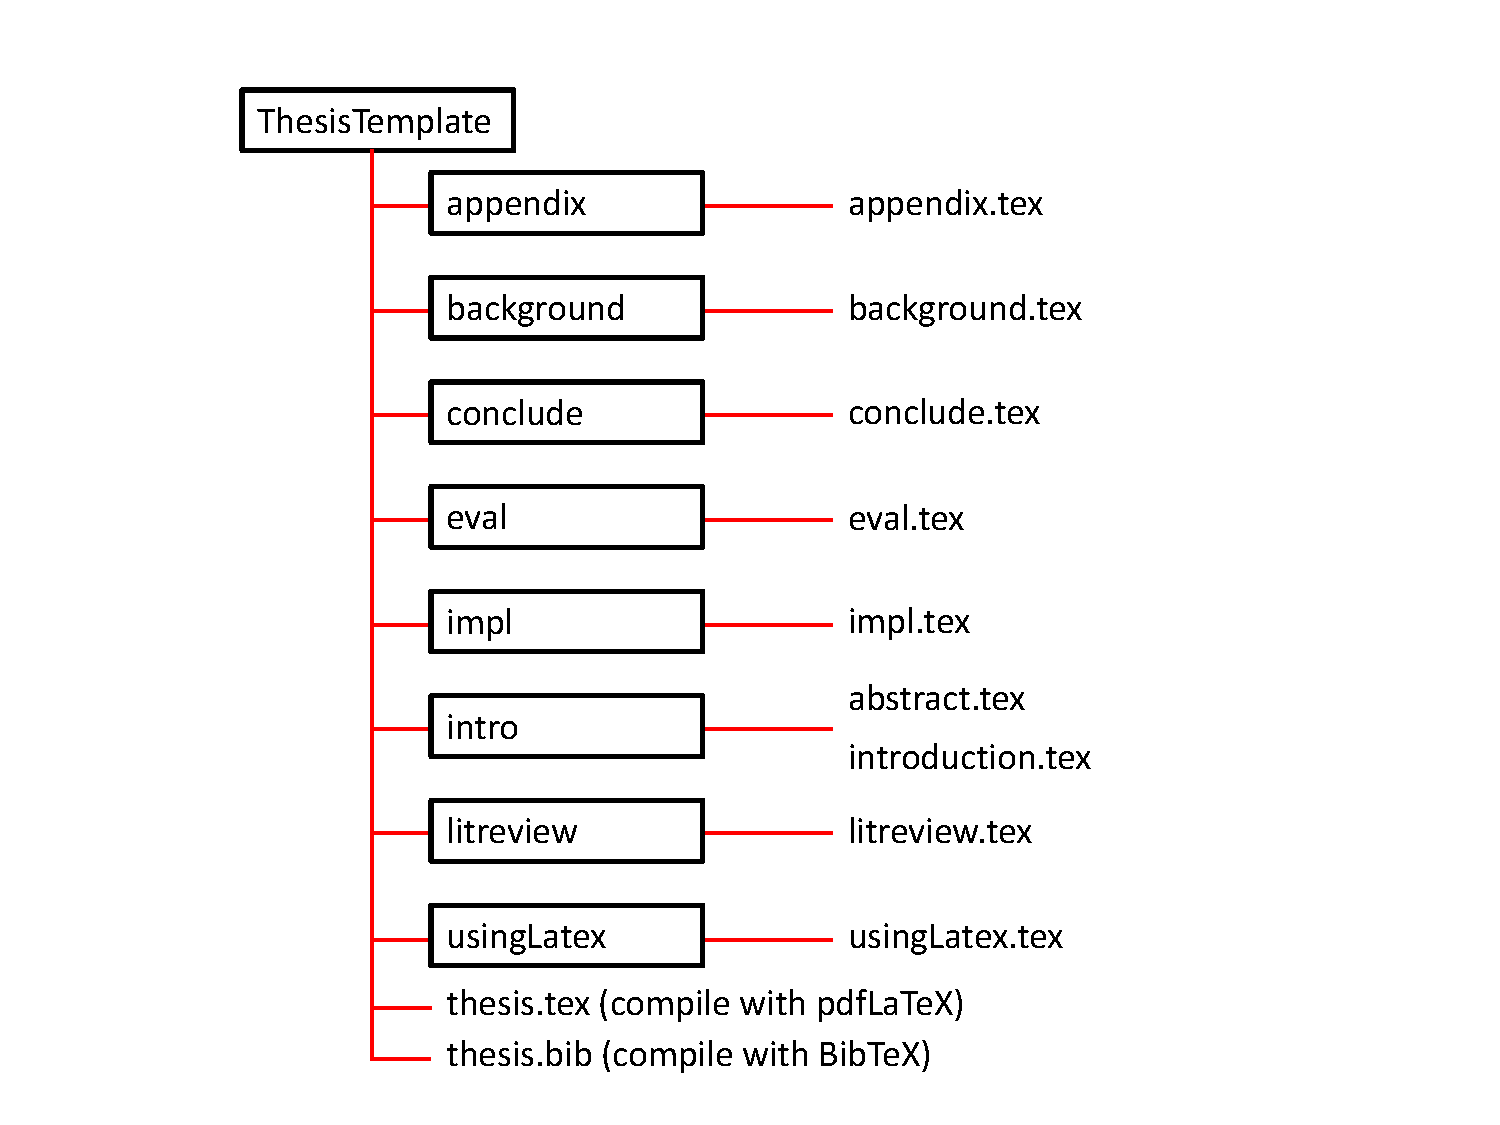
\includegraphics[width=.9\linewidth]{appendix/images/TemplateStructure.pdf}
\caption{Thesis Template Folder and \latex File Structure}
\label{fig:append:TemplateStructure}
\end{figure}

\begin{sidewaystable}
\begin{center}
   \begin{tabular}{lllllllll} 
   \toprule
   \textbf{Heading 1} & \textbf{Heading 2}  & \textbf{Heading 3}  & \textbf{Heading 4}  & \textbf{Heading 5}  & \textbf{Heading 6}  & \textbf{Heading 7}  & \textbf{Heading 8}  & \textbf{Heading 9}  \cr
   \midrule
   AAAA & BBBB & CCCC & DDDD & EEEE & FFFF & XXXX & YYYY & ZZZZ \cr 
   AAAA & BBBB & CCCC & DDDD & EEEE & FFFF & XXXX & YYYY & ZZZZ \cr 
   AAAA & BBBB & CCCC & DDDD & EEEE & FFFF & XXXX & YYYY & ZZZZ \cr 
   AAAA & BBBB & CCCC & DDDD & EEEE & FFFF & XXXX & YYYY & ZZZZ \cr 
   AAAA & BBBB & CCCC & DDDD & EEEE & FFFF & XXXX & YYYY & ZZZZ \cr 
   AAAA & BBBB & CCCC & DDDD & EEEE & FFFF & XXXX & YYYY & ZZZZ \cr 
   \bottomrule
   \end{tabular}
\caption[A Short Caption for the Table]{
	A much longer caption that will not be listed in the list of tables page.
}
\label{tab:sidewaysTable}
\end{center}
\end{sidewaystable}

\begin{sidewaysfigure}
\centerline{\includegraphics[width=7in]{appendix/images/samplepng}}
\caption[A Sideways Figure]{
	A much longer caption that will not be listed in the list of figures page.
}
\label{fig:sidewaysFigure}
\end{sidewaysfigure}

\chapter{Presentation Slides}
One can readily prepare presentation slides using PowerPoint or Keynote. Saving / Exporting the slides as a pdf document allows for it to be easily incorporated into this template. Each slide will be scaled to 0.45 of the \textbackslash textwidth, individual pages of the file can be accessed via the page=x option of \textbackslash includegraphics.  


\begin{figure}[H]
\parbox{74.mm}{
    \centering
    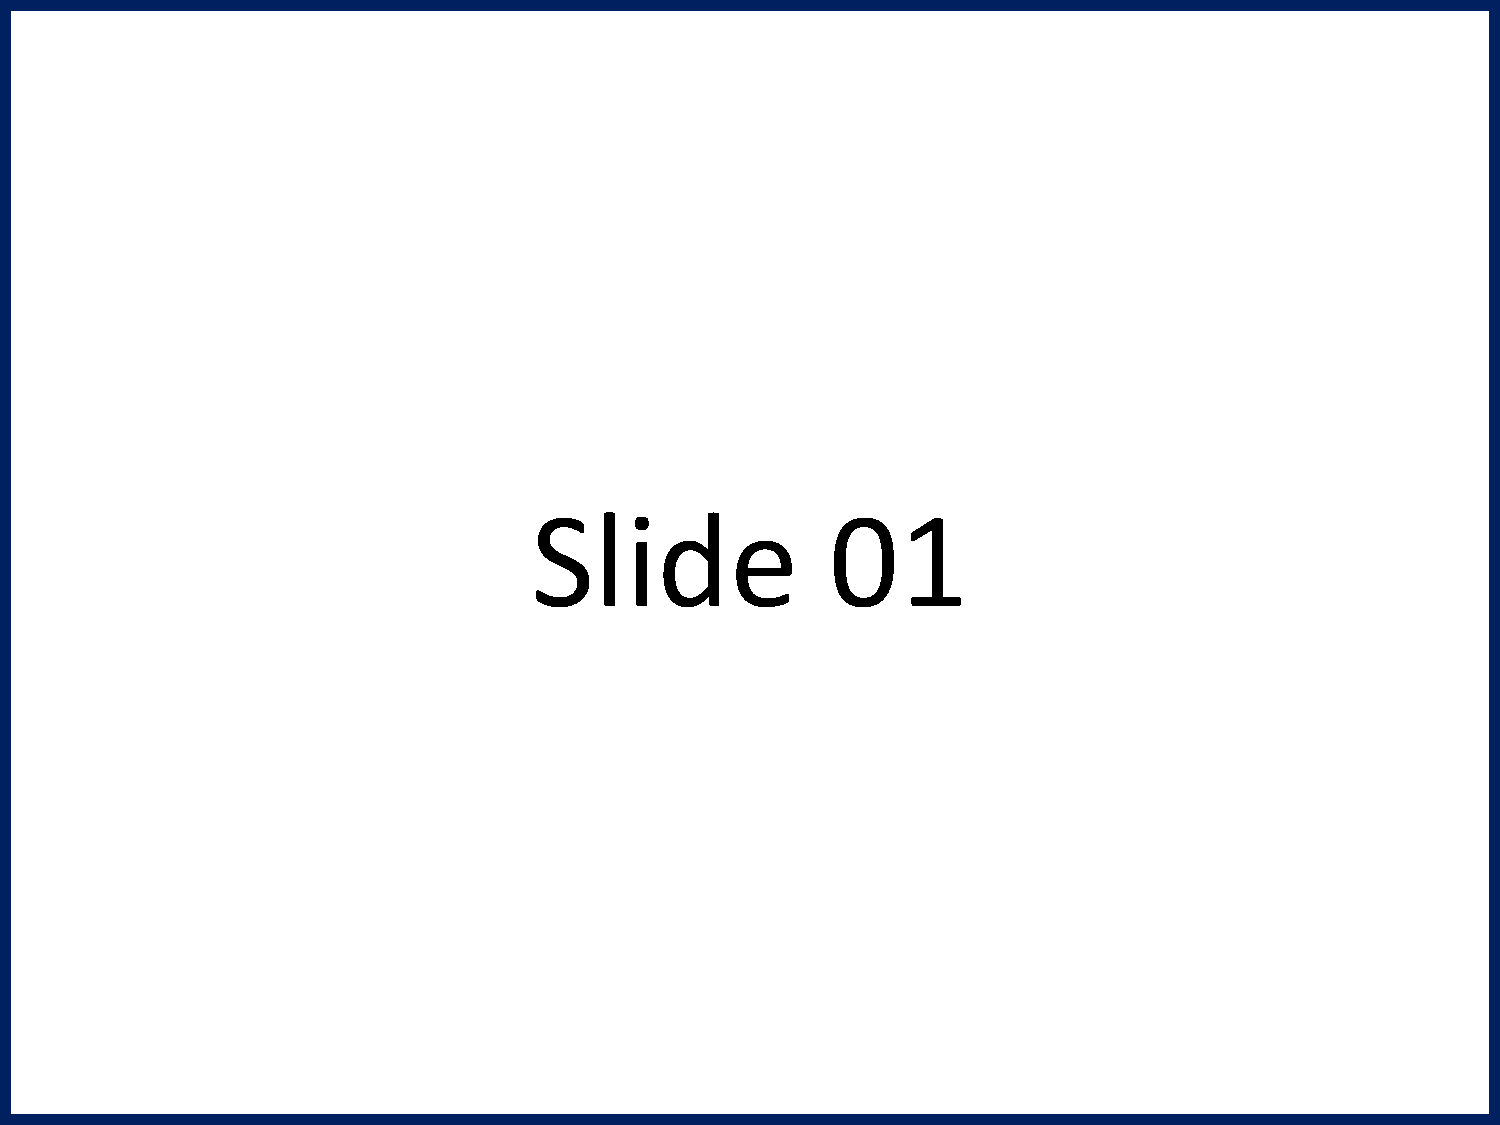
\includegraphics[width=0.45\textwidth,page=1]{appendix/images/PresentationSlides}
    \caption*{Slide 1}
}
    \parbox{74.mm}{
    \centering
    \includegraphics[width=0.45\textwidth,page=2]{appendix/images/PresentationSlides}
    \caption*{Slide 2}
}
\end{figure}

\begin{figure}[H]
\parbox{74.mm}{
    \centering
    \includegraphics[width=0.45\textwidth,page=3]{appendix/images/PresentationSlides}
    \caption*{Slide 3}
}
    \parbox{74.mm}{
    \centering
    \includegraphics[width=0.45\textwidth,page=4]{appendix/images/PresentationSlides}
    \caption*{Slide 4}
}
\end{figure}

\begin{figure}[H]
\parbox{74.mm}{
    \centering
    \includegraphics[width=0.45\textwidth,page=5]{appendix/images/PresentationSlides}
    \caption*{Slide 5}
}
    \parbox{74.mm}{
    \centering
    \includegraphics[width=0.45\textwidth,page=6]{appendix/images/PresentationSlides}
    \caption*{Slide 6}
}
\end{figure}

\begin{figure}[H]
\parbox{74.mm}{
    \centering
    \includegraphics[width=0.45\textwidth,page=7]{appendix/images/PresentationSlides}
    \caption*{Slide 7}
}
    \parbox{74.mm}{
    \centering
    \includegraphics[width=0.45\textwidth,page=8]{appendix/images/PresentationSlides}
    \caption*{Slide 8}
}
\end{figure}

\begin{figure}[H]
\parbox{74.mm}{
    \centering
    \includegraphics[width=0.45\textwidth,page=9]{appendix/images/PresentationSlides}
    \caption*{Slide 9}
}
    \parbox{74.mm}{
    \centering
    \includegraphics[width=0.45\textwidth,page=10]{appendix/images/PresentationSlides}
    \caption*{Slide 10}
}
\end{figure}

\chapter{Project Log}

The following is a weekly summary of the work carried during the development of this body of work. It covers tasks that were completed, tutorials that were worked through, articles that were read and summaries of discussions / meetings held with the project supervisor and other third parties. 

\section*{Week Beginning: Monday 26/09/2022}

First week working on the project. Had a meeting with supervisor and discussed some of the issues related to the project. The first deliverable is due for the end of next week (project outline \& ethics form). 

\begin{itemize}
  \item Downloaded and Installed \latex (MikTeX full install) and TeXmaker. 
  \item Started to get to grips with the \latex system by making simple modifications to the template and editing the project log.
  \item Developed a Mind Map to clarify understanding of project elements.
  \item Prepared an initial draft of project plan in the form of a Gantt chart. 
  \item Prepared and revised draft of project proposal. 
  \item Downloaded and read half a dozen BSc \& MSc Project Reports to see the general format and expected content. A list of the reports could be included here.
  \item Started learning how to use some API's needed for the project. 
  \item Looked on the University Library website for link to the ``Databases'' area providing access to repositories such as IEEE Explore and ACM Digital Library. 
\end{itemize}




\end{document} % NOTE: END of document, nothing after this point
